\section{Beweis der Funktionsfähigkeit}
In der Theorie funktionierte dieses Konstrukt bereits in Kapitel \ref{architektur}. Im Folgenden soll gezeigt werden, dass das entworfene Konstrukt aber auch in der Praxis relevante Werte liefert. Hierzu wird das in Kapitel \ref{numerschiesBeispiel} herangezogen, sowie ein standardisiertes Beispiel aus dem Themenbereich des \ac{TSP}, nämlich das a280-Problem - also eine Problemstellung mit 280 Städten.

\subsection{numerisches Beispiel}

\begin{figure}[h]
	\centering
	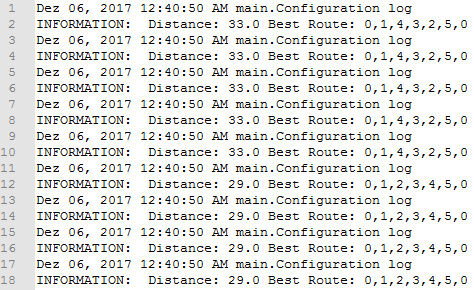
\includegraphics[width=0.6\linewidth]{images/numerischErgebnis.png}
	\caption{Ausschnitt der Log-Datei bei der Berechnung des numerischen Beispiels aus \ref{numerschiesBeispiel}}
	\label{numerischBeweis}
\end{figure}

\subsection{a280 drilling problem}

\begin{figure}[h]
	\centering
	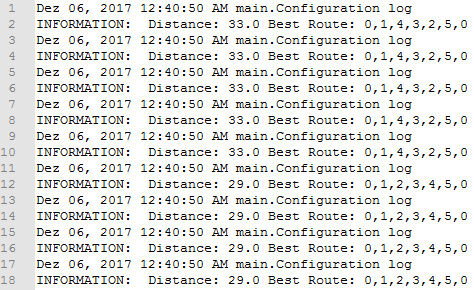
\includegraphics[width=0.6\linewidth]{images/numerischErgebnis.png}
	\caption{Ausschnitt der Log-Datei bei der Berechnung des ``a280 drilling problem''}
	\label{drillingBeweis}
\end{figure}